\section{Rain Augmentation}
\label{sec:rain_aug}

\begin{figure}
\centering
\includegraphics[width=\linewidth]{figures/pipeline_v3_img.pdf}
\caption{\textbf{Physics-Based Rendering for rain augmentation.} We use particles simulation together with depth and illumination estimation to render arbitrarily controlled rainfall on clear images.}
\label{fig:pipeline}
\end{figure}

Broadly speaking, synthesizing rain on images can be achieved using two seemingly antagonistic methods: 1)~physics-based rendering~(PBR) methods~\cite{halimeh2009raindrop,garg2006photorealistic}, which explicitly model the dynamics and the radiometry of rain drops in images; or 2)~learning-based image-to-image translation approaches~\cite{zhu2017unpaired,huang2018multimodal}, which train deep neural networks to ``translate'' an image into its rainy version. While completely different, we argue both these methods offer complementary advantages. On one hand, physics-based approaches are accurate, controllable, can simulate a wide variety of imaging conditions, and do not require any training data. On the other hand, learning-based approaches can realistically simulate important visual cues such as wetness, cloud cover, and overall gloominess typically associated with rainy images. 

In this paper, we propose to first explore the use of both techniques independently, then to \emph{combine} them into a hybrid approach. This section thus first describes our PBR approach~(sec.~\ref{sec:rain_pbr}), followed by the image-to-image translation with a GAN~(sec.~\ref{sec:rain_gan}), and concludes with the hybrid combination of the two GAN+PBR~(sec.~\ref{sec:rain_hybrid}).

\subsection{Physics-Based Rendering (PBR)}
\label{sec:rain_pbr}

Taking inspiration from the vast literature on rain physics, \cite{marshall1948distribution,van1997numerical,garg2007vision,narasimhan2002vision} we simulate the rain appearance in an arbitrary image with the approach summarized in fig.~\ref{fig:pipeline}. Based on the estimated scene depth, a fog-like attenuation layer is first generated. Individual rain streaks are subsequently generated, and composited with the fog-like layer. The final result is blended in the original image to create a realistic, physics-based and controllable rainfall rate. 
 
\subsubsection{Fog-like rain}
\label{sec:rendering.fog-like}

Following the definition of \cite{garg2007vision}, fog-like rain is the set of drops that are too far away and that project on an area smaller than 1 pixel. In this case, a pixel may even be imaging a large number of drops, which causes optical attenuation~\cite{garg2007vision}.
In practice, most drops in a rainfall are actually imaged as fog-like rain\footnote{Assuming a stationary camera with KITTI calibration~\cite{Geiger2013IJRR}, we computed that only 1.24\% of the drops project on 1+ pixel in 50~mm/hr rain, and 0.7\% at 5~mm/hr. This follows logic: the heavier the rain, the higher the probability of having large drops.}, though their visual effect is less dominant.

We render the volumetric attenuation using the model described in \cite{weber2015multiscale} where the per-pixel attenuation $I_\text{att}$ is expressed as the sum of the extinction $L_\text{ext}$ caused by the volume of rain and the airlight scattering $A_\text{in}$ that results of the environmental lighting. Using equations from \cite{weber2015multiscale} to model the attenuation image at pixel $\mathbf{x}$ we get
\begin{equation}
\label{eq:render-foglike}
I_\text{att}(\mathbf{x}) = I L_\text{ext}(\mathbf{x}) + A_\text{in}(\mathbf{x}) \,,
\end{equation}
where
\begin{equation}
\begin{split}
L_\text{ext}(\mathbf{x}) &= e^{-0.312R^{0.67}d(\mathbf{x})}  \,, \\
A_\text{in}(\mathbf{x})  &= \beta_\text{HG}(\theta) \bar{E}_\text{sun} (1 - L_\text{ext}(\mathbf{x}))  \,.
\end{split}
\end{equation}
Here, $R$ denotes the rainfall rate $R$ (in mm/hr), $d(\mathbf{x})$ the pixel depth, $\beta_\text{HG}$ the standard Heynyey-Greenstein coefficient, and $\bar{E}_\text{sun}$ the average sun irradiance which we estimate from the image-radiance relation~\cite{horn1986robot}.

\begin{figure}[!t]
 \centering
 \footnotesize
 \subfloat[Drop FOV]{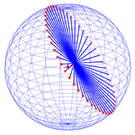
\includegraphics[width=0.24\linewidth]{figures/drop_fov_sphere.png}\label{fig:drop_cam_fov_fov}}\hspace{0.05\linewidth}
 \subfloat[Environment map estimation~\cite{Cameron2005}]{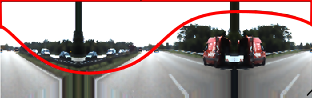
\includegraphics[width=0.7\linewidth]{figures/env_map_drop_fov.png}\label{fig:drop_cam_fov_envmap}}
 \vspace{.25em}
 \caption{
     \textbf{Estimation of raindrop photometry.} To estimate the photometric radiance of a drop, we integrate the lighting environment map over the 165$^{\circ}$ drop field of view \protect\subref{fig:drop_cam_fov_fov} relying on an estimate of the environment map $E$ shown in \protect\subref{fig:drop_cam_fov_envmap}. The projected field of view ($F$) of the drop is outlined in red.
 }
 \label{fig:drop_cam_fov}
\end{figure}


\subsubsection{Simulating the physics of raindrops}
\label{sec:raindrop-position}

We use the particles simulator of \cite{de2012fast} to compute the position and dynamics of all raindrops greater than 1~mm for a given fall rate\footnote{The distribution and dynamics of drops vary on earth due to gravity and atmospheric conditions. We selected here the broadly used physical models recorded in Ottawa, Canada~\cite{marshall1948distribution,atlas1973doppler}.}. 
The simulator outputs the position and dynamics (start and end points of streaks) of all visible rain drops in both world and image space, and accounts for intrinsic and extrinsic camera calibration.

\subsubsection{Rendering the appearance of a rain streak}
\label{sec:rwa_appearance}

While ray casting allows exact modeling of drops photometry, this comes at very high processing cost and is virtually only possible in synthetic scenes where the geometry and surface materials are perfectly known~\cite{rousseau2006realistic,halimeh2009raindrop}. What is more, drops oscillate as they fall, which creates further complications in modeling the light interaction. Instead, we rely on the raindrop appearance database of Garg and Nayar~\cite{garg2007vision}, which contains the individual rain streaks radiance when imaged by a stationary camera. For each drop, the streak database also models 10 oscillations due to the airflow, which accounts for much greater realism than Gaussian modeling~\cite{barnum2010analysis}. 

To render a raindrop, we first select a rain streak $S \in \mathcal{S}$ from the streak database $\mathcal{S}$ of \cite{garg2006photorealistic}, which contains 20 different streaks (each with 10 different oscillations) stored in an image format. 
We select the streak that best matches the final drop dimensions (computed from the output of the physical simulator), and randomly select an oscillation. 

The selected rain streak $S$ is subsequently warped to match the drop dynamics from the physical simulator: 
\begin{equation}
S' = \mathcal{H}(S) \,,
\label{eq:drop_warp}
\end{equation}
where $\mathcal{H}(\cdot)$ is the homography computed from the start and end points in image space given by the physical simulator and the corresponding points in the database streak image.

\subsubsection{Computing the photometry of a rain streak}
\label{sec:photometry-rainstreak}

Computing the photometry of a rain streak from a single image is impractical because drops have a much larger field of view than common cameras ($165^\circ$ vs approx. 70--100$^\circ$). To render a drop accurately, we must therefore estimate the environment map (spherical lighting representation) around that drop. 
Sophisticated methods could be used~\cite{holdgeoffroy-cvpr-17,holdgeoffroy-cvpr-19,zhang-cvpr-19} but we employ~\cite{Cameron2005} which approximates the environment map through a series of simple operations on the image. 

From each camera relative 3D drop position, we compute the intersection $F$ of the drop field of view with the environment map $E$, assuming a 10m constant scene distance.
The process is depicted in fig.~\ref{fig:drop_cam_fov}, and geometrical details are provided in appendix~\ref{sec:app-geom-drop-fov}.
Note that geometrically exact drop field of view estimation requires location-dependent environment maps, centered on each drop. However, we consider the impact negligible since drops are relatively close to the camera center compared to the sphere radius used\footnote{We computed that, for KITTI, 98.7\% of the drops are within 4~m from the camera center in a 50~mm/hr rainfall rate. Therefore, computing location-dependent environment maps would not be significantly more accurate,  while being of very high processing cost.}. 

Since a drop refracts 94\% of its field of view radiance and reflects 6\% of the entire environment map radiance~\cite{garg2007vision}, we multiply the streak appearance with a per-channel weight: 
\begin{equation}
S' = S' (0.94 \bar{F} + 0.06 \bar{E}) \,,
\label{eq:photometry_rainstreak}
\end{equation}
where $\bar{F}$ is the mean of the intersection region $F$, and $\bar{E}$ is the mean of the environment map $E$. 


\begin{figure}[!t]
 \centering
 \footnotesize
 \setlength{\tabcolsep}{0.02cm}
 \renewcommand{\arraystretch}{0.5}
 \begin{tabular}{ccc}
  \multirow{1}{*}[1.35cm]{\rotatebox{90}{Ground truth}}&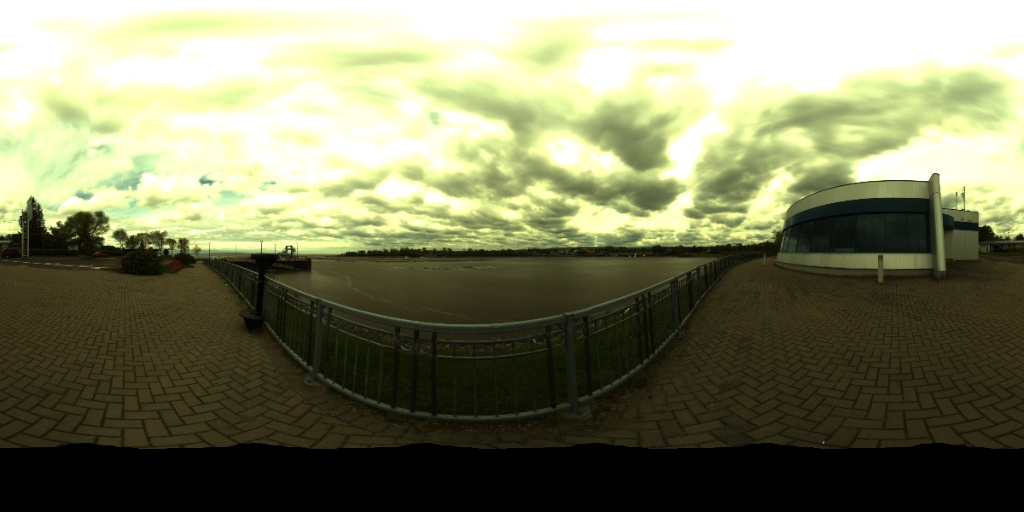
\includegraphics[width=0.31\linewidth, height=0.19\linewidth]{figures/results/panos_rain_comparison/1_envmap_pano_lr.jpg}&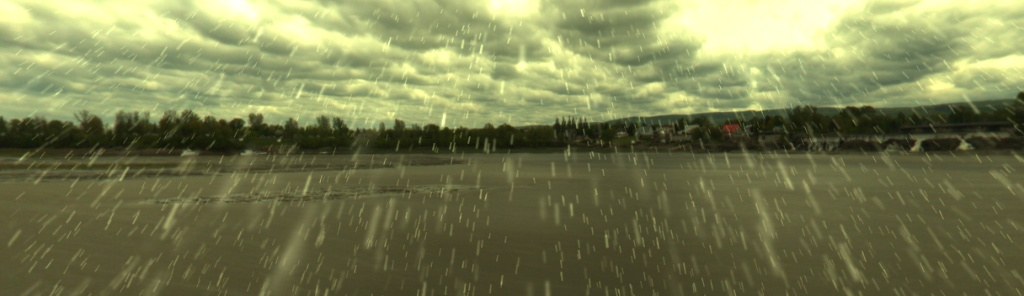
\includegraphics[width=0.65\linewidth]{figures/results/panos_rain_comparison/1_pano_lr.jpg}\\
  \multirow{1}{*}[0.85cm]{\rotatebox{90}{Ours}}&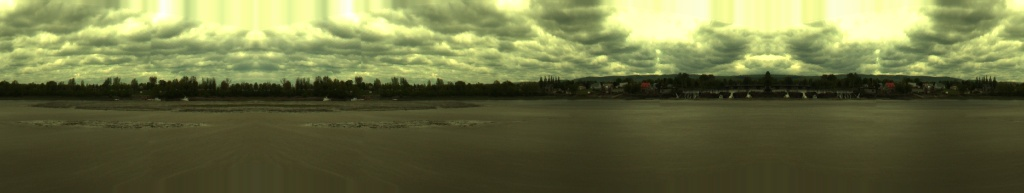
\includegraphics[width=0.31\linewidth, height=0.19\linewidth]{figures/results/panos_rain_comparison/1_envmap_ours_lr.jpg}&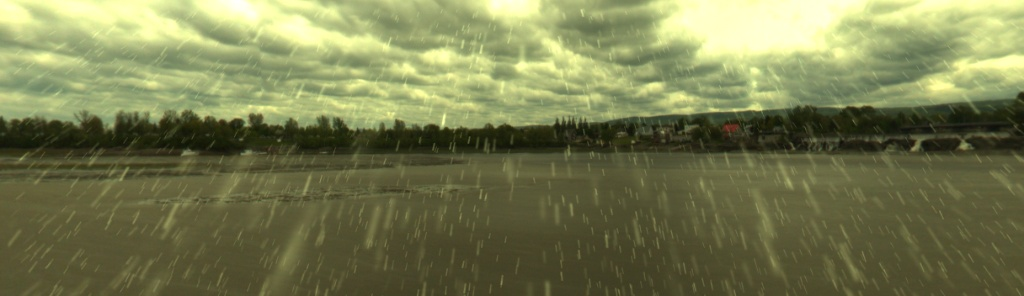
\includegraphics[width=0.65\linewidth]{figures/results/panos_rain_comparison/1_ours_lr.jpg}\vspace{0.05in}\\
  \multirow{1}{*}[1.35cm]{\rotatebox{90}{Ground truth}}&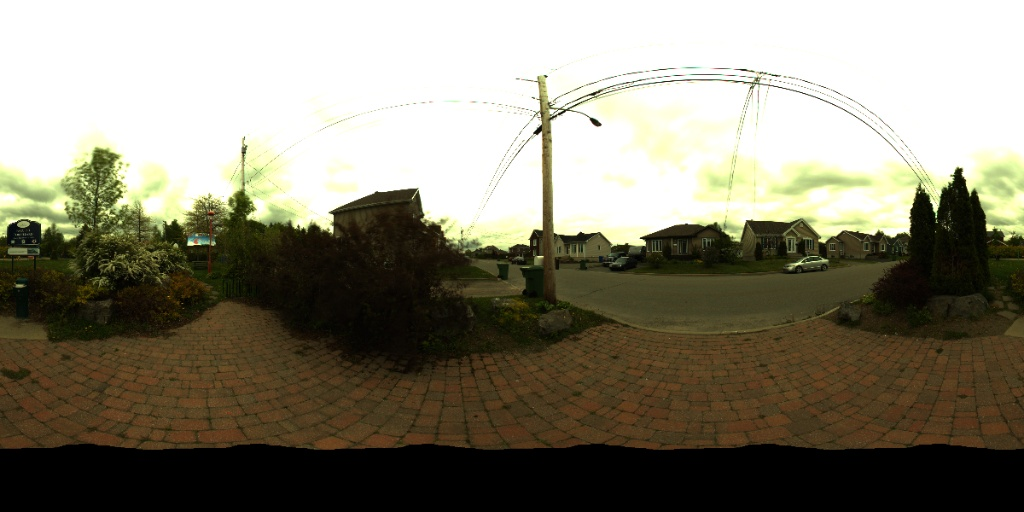
\includegraphics[width=0.31\linewidth, height=0.19\linewidth]{figures/results/panos_rain_comparison/12_envmap_pano_lr.jpg}&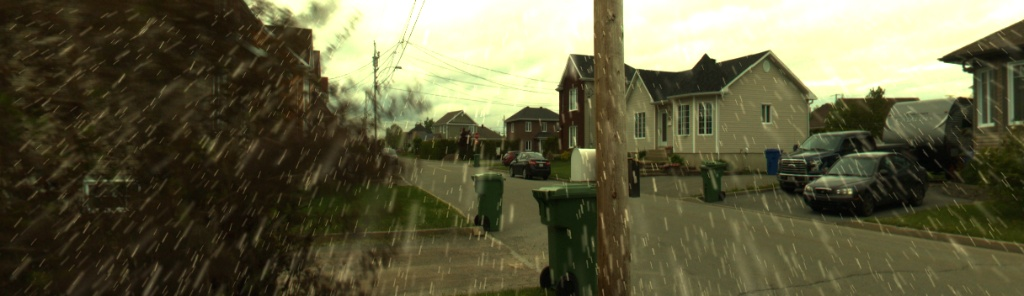
\includegraphics[width=0.65\linewidth]{figures/results/panos_rain_comparison/12_pano_lr.jpg}\\
  \multirow{1}{*}[0.85cm]{\rotatebox{90}{Ours}}&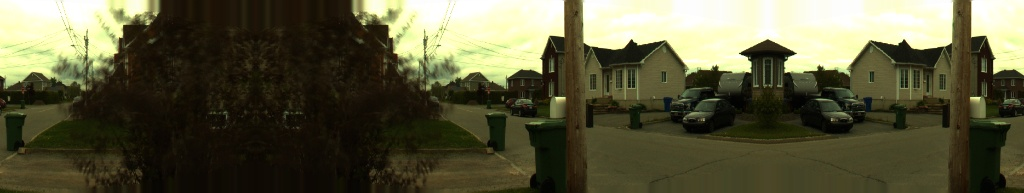
\includegraphics[width=0.31\linewidth, height=0.19\linewidth]{figures/results/panos_rain_comparison/12_envmap_ours_lr.jpg}&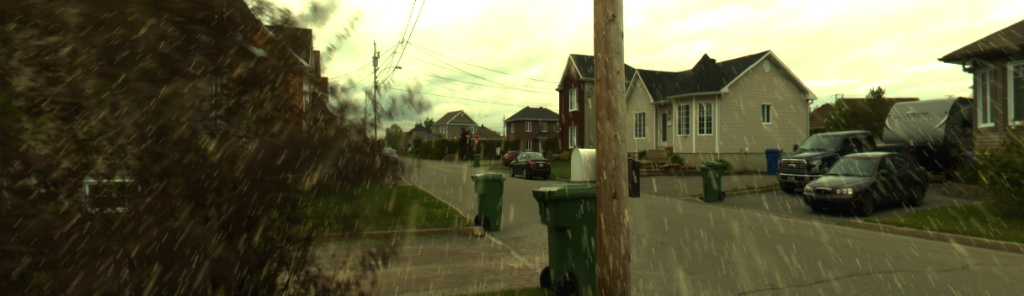
\includegraphics[width=0.65\linewidth]{figures/results/panos_rain_comparison/12_ours_lr.jpg}\\
  & Environment map & Our synthesized rain (50mm/hr) \\
 \end{tabular}
 \caption{\textbf{Photometric validation of rain.} Rain rendering using ground truth illumination or our approximated environment map. 
 From HDR panoramas~\cite{holdgeoffroy-cvpr-19}, we first extract limited field of view crops to simulate the point of view of a regular camera. Then, 50mm/hr rain is rendered using either (rows 1, 3) the ground truth HDR environment map or (rows 2, 4) our environment estimation. The environment maps are shown as reference on the left. While our approximated environment maps differ from the ground truth, they are sufficient to generate visually similar rain in images.}
 \label{fig:pano_ours_comparison}
\end{figure}

\subsubsection{Compositing a single rain streak on the image}
\label{sec:rendering.streak-compositing}

Now that the streak position and photometry were determined from the physical simulator and the environment map respectively, we can composite it onto the original image. 
First, to account for the camera depth of field, we apply a defocus effect following~\cite{potmesil1981lens}, convolving the streak image $S'$ with the circle of confusion\footnote{The circle of confusion $C$ of an object at distance $d$, is defined as: $C = \frac{(d - f_{\text{p}}) f^2}{d(f_{\text{p}} - f) f_{\text{N}}}$ with $f_\text{p}$ the focus plane, $f$ the focal and $f_\text{N}$ the lens f-number. $f$ and $f_\text{N}$ are from intrinsic calibration, and $f_\text{p}$ is set to 6~m.} $C$, that is: $S' = S' * C$. 

We then blend the rendered drop with the attenuated background image $I_{\text{att}}$ using the photometric blending model from \cite{garg2007vision}. Because the streak database and the image $I$ are likely to be imaged with different exposures, we need to correct the exposure to match the imaging system used in~$I$.
Suppose a pixel $\mathbf{x}$ of the image $I$ and $\mathbf{x}'$ the overlapping coordinates in streak $S'$, the composite is obtained with
\begin{equation}
I_{\text{rain}}(\mathbf{x}) = \frac{T - S'_{\alpha}(\mathbf{x'})\tau_1}{T}I_{\text{att}}(\mathbf{x}) + S'(\mathbf{x'})\frac{\tau_1}{\tau_0}\,,
\label{eq:rain_blending}
\end{equation}
where $S'_{\alpha}$ is the alpha channel\footnote{While \cite{garg2006photorealistic} does not provide an alpha channel, the latter is easily computed since drops were rendered on black background in a white ambient lighting.} of the rendered streak, $\tau_0 = \sqrt{10^{-3}} / 50$ is the time for which the drop remained on one pixel in the streak database, and $\tau_1$ the same measure according to our physical simulator. We refer to appendix~\ref{sec:app-comp_diff_exp} for details.

\subsubsection{Compositing rainfall on the image}

The rendering of rainfall of arbitrary rates in an image is done in three main steps:
1)~the fog-like attenuated image $I_{\text{att}}$ is rendered (eq.~\ref{eq:render-foglike}), 
2)~the drops outputted by the physical simulator are rendered individually on the image (eq.~\ref{eq:rain_blending}),
3)~the global luminosity average of the rainy image denoted $I_{\text{rain}}$ is adjusted. 
While rainy events usually occur in cloudy weather which consequently decreases the scene radiance, a typical camera imaging system adjusts its exposure to restore the luminosity. Consequently, we adjust the global luminosity factor so as to restore the mean radiance, and preserves the relation $\bar{I} = \bar{I}_{\text{rain}}$, where the overbar denotes the intensity average.


\paragraph{Photometric validation.} A limitation of our physical pipeline is the lighting estimation which impacts the photometry of the rain. 
To measure its effect, in fig.~\ref{fig:pano_ours_comparison} we compare the same rain rendered with our estimated environment map or ground truth illumination obtained from high dynamic range panoramas~\cite{holdgeoffroy-cvpr-19}. 
Overall, our estimation differs from ground truth when the scene is not radially symmetric but we observe that it produces visually similar rain in images.


\subsection{Image-to-image translation (GAN)}
\label{sec:rain_gan}

While our physic-based rendering generates realistic rain streaks and fog-like rain effect, it ignores major rainy characteristics such as wetness, reflections, clouds and thus may fail at conveying the overall look of a rainy scene. Conversely, generative adversarial networks (GAN) excel at learning such visual characteristics as they constitute strong signals for the discriminator in the learning process.

We further learn the $\text{clear}\mapsto{}\text{rain}$ mapping with CycleGAN~\cite{zhu2017unpaired} from a set of unpaired clear/rain images.
We train our model with the $256\times256$ architecture from~\cite{zhu2017unpaired} on images of input size $448\times256$. The generator is similar to~\cite{johnson2016perceptual} with 2 downsampling blocks followed by 9 ResNet blocks and 2 upsampling blocks. The discriminator is a simple 3 hidden layers ConvNet similar to the one used in PatchGAN~\cite{isola2017image}. The model is optimized for 40 epochs with Adam, using batch size of 1, a learning rate of 0.0002, and $\beta = \left\{ 0.5, 0.999 \right\}$. 

\subsection{Combining GAN and PBR}
\label{sec:rain_hybrid}

\begin{figure}
 \centering
 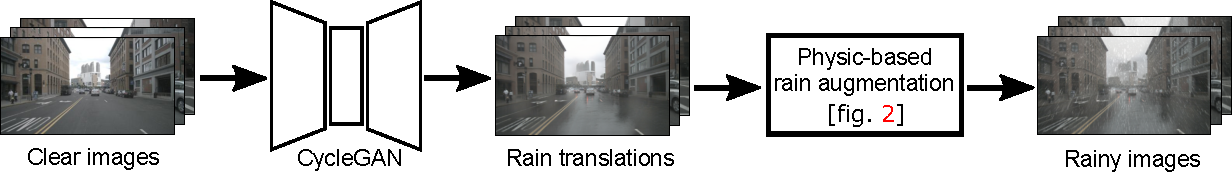
\includegraphics[width=\linewidth]{figures/pipeline_hybrid_v2_img.pdf}
 \caption{\textbf{GAN+PBR rain-augmentation architecture.} In this hybrid approach, clear images are first translated into rain with CycleGAN~\cite{zhu2017unpaired} and subsequently augmented with rain streaks with our PBR pipeline (see fig.~\ref{fig:pipeline}).}
 \label{fig:hybrid_architecture}
\end{figure}

We combine both the PBR- and the GAN-based rain generation methods together, simply by first translating the image to its rainy version with the GAN, then compositing the rain layer onto the resulting image using PBR (see fig.~\ref{fig:hybrid_architecture}). The sun irradiance estimation $\bar{E}_{sun}$ (sec.~\ref{sec:rendering.fog-like}) of the ``translated'' image is typically darker, which, in turn, makes the fog-like rain more realistic. The estimated environment map is also darker and, consequently, so is its mean value $\bar{E}$. The appearance of rain streaks will thus remain coherent with their environment.

Since rain streaks smaller than 1px in diameter are ignored before the rendering and instead generated as fog-like rain (sec.~\ref{sec:rendering.fog-like}), we need to apply the PBR renderer at full resolution by upsampling the output of the GAN to the image original size. Once the rain rendering is complete, we downsample the augmented image at $448\times256$.
We further refer to this hybrid rendering as GAN+PBR.
